\documentclass{book}
\usepackage{float}
\usepackage{graphicx}
\usepackage{amsmath}
\usepackage{amssymb}
\title{Figures Theoretical Mechanics}
\author{Felix Claeys, Brecht Verbeken, Simon Verbruggen}
\begin{document}
\maketitle
\section*{4.4 Euler angles}
\begin{figure}[H]
\centering
\includegraphics{CH4/4.4_Euler_angles/standalone.pdf}
\caption{The rotations defining the Eulerian angles.}
\end{figure}

\section*{4.8 Infinitesimal rotations}
\begin{figure}[H]
\centering
\includegraphics{CH4/4.8_Infinitesimal_rotations/standalone.pdf}
\caption{Change in a vector $\boldsymbol{r}$ produced by an infinitesimal clockwise rotation $\mathrm{d}\Phi$ of the vector.}
\end{figure}

\end{document}